% !TEX root = ./ICDE14_conf_full_296.tex
\section{\hl{Algorithms for selection problem}}
\label{sec:algorithms}

\hl{As mentioned in Section}~\ref{sec:filtering}\hl{, we solve the multi-scale selection problem using the ladder approach. For each of the }$\mathcal{Z}$\hl{ zoom levels, we generate and solve a separate instance of the selection optimization problem }(Section~\ref{sec:optimizationmodel}). \hl{The solution gives us the records that should be deleted from zoom-level $i$. The remaining records are (conceptually) copied to zoom level $i-1$, unless we have reached the last zoom level ($i=1$). This approach is illustrated schematically in Figure}~\ref{fig:algorithmic-framework}.

%\marcos{The algorithmic framework is not for multi-scale filtering, but for iterated single-scale filtering? Seems to me that these two are not the same thing.}
%\martin{Well, we do indeed solve (approximately) the multi-scale problem by iterated single-scale filtering, so I would say that this is okay. However, we don't have any good lower bound for the multi-scale problem, only for each of the single-scale problems.}

\begin{figure}[htbp]
\begin{center}
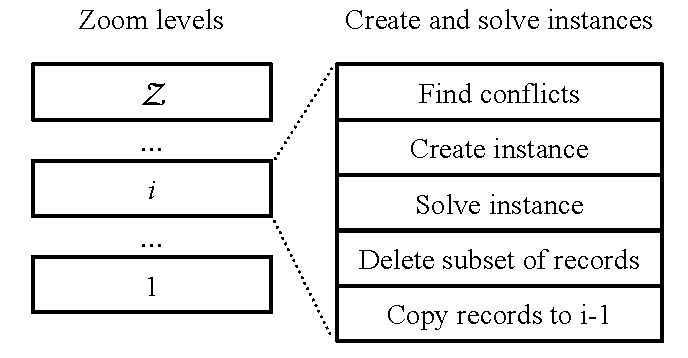
\includegraphics[scale=.6]{figs/cvl_stages.pdf}
\caption{Algorithmic framework: At each zoom level $i \in \{ 1, \ldots, \mathcal{Z} \}$ we solve a selection optimization problem. In the ladder approach, the problem is solved for the ``highest'' zoom level first.}
\label{fig:algorithmic-framework}
\end{center}
\end{figure}

Below we describe two different heuristic algorithms for solving the selection optimization problem. Let $n=|C|$ be the number of conflicts (or elements in the set multicover problem), and let $m=|R|$ be the number of records (or sets in the set multicover problem). Recall that $R_c \subseteq R$ is the set of records in conflict $c \in C$. The largest number of records in any conflict is $f = \max_{c \in C} |R_c|$, and is called the \emph{maximum frequency}.

\subsection{Static greedy algorithm (SGA)}
\label{sec:algorithms:sga}

In this algorithm, we consider each conflict $c \in C$ in turn, and simply choose the $\lambda_c$ records with minimum weight from the records $R_c$ --- independently of what has been chosen earlier. If the sets $R_c$ are disjoint, the algorithm is clearly optimal. However, in general no approximation guarantee can be provided. The algorithm runs in $O(n f \log f)$ time, as we just need to sort the records by weight for each conflict set; alternatively we can sort all records by weight in $O(m \log m)$ time and pick the minimum weight records from the conflicts in linear time in the total number of records in all conflict sets.

\subsection{LP-based greedy algorithm (LPGA)}
\label{sec:algorithms:lpga}

In this algorithm, we first solve a linear programming (LP) relaxation of the set multicover problem. This LP-problem is obtained by relaxing the constraint $x_r \in \{0, 1\}$ to $0 \leq x_r \leq 1$. Then we choose all records $r \in R$ for which the LP-solution variable $x_r$ is at least $1 / f$. Intuitively, we round up to 1 all fractional values that are large enough; the remaining fractional variables are rounded down to 0.

This algorithm provides a feasible solution to the selection optimization problem, and the approximation guarantee is $f$~\cite{vazirani2001approximation}; thus, if $f$ is small, the algorithm provides a good approximation guarantee. As the LP-problem can be solved in polynomial time, the complete algorithm is polynomial.

%\subsection{Dynamic greedy algorithm (DGA)}

%Described in Vazirani 13.2.1. @Martin: Please write here.

%\marcos{I would only introduce DGA if it is actually evaluated in the experiments.}

